\section{Segunda consigna: gráficos y análisis}
%Aparte de los gráficos detallados en este informe existe una carpeta llamada ”grafos” donde se pueden visualizar los grafos de cada red analizada.

\subsection{Red con información previa}
Para tener una base de partida sólida sobre la cual extrapolar, la primera captura que realizamos fue en una red hogareña de uno de los integrantes 
del grupo en la que cual pudieramos determinar de manera feaciente cada uno de los dispositivos que se encontraban en la red. Suponemos que el host
con una mayor interacción en envíos y recepción de paquetes $ARP$ será el router dado que todos los dispositivos buscarían comunicarse directamente
con él para acceder a Internet. Con respecto los demás dispositivos suponemos una interacción distribuida, donde se envían espacialmente paquetes $ARP$
en caso de querer establer alguna conexión o actualizar sus datos.\\

Durante la escucha, cada uno de los dispositivos concervó la siguente ip:\\
\begin{table}[htb]
\begin{center}
\begin{tabular}{|l|l|}
\hline
IP & Host \\
\hline \hline
192.168.1.1 & Router \\ \hline
192.168.1.3 & Celular (wifi) \\ \hline
192.168.1.6 & Computadora (wifi)  \\ \hline
192.168.1.10 & Computadora (wifi) \\ \hline
192.168.1.36 & Computadora (cable ethernet) \\ \hline
\end{tabular}
\caption{Información previa - Red Doméstica}
\label{tabla informacion}
\end{center}
\end{table}

%192.168.1.1 -> ip del router
%192.168.1.3 -> ip de celular (wifi)
%192.168.1.6 -> ip de mi computadora (wifi)
%192.168.1.36 -> computadora conectada por cable ethernet
%192.168.1.10 -> computadora conectada (wifi) con Windows 7

Lo que pudimos observar simulando la fuente $S$ durante $4$ horas en esta red fue lo siguiente:\\
%\begin{figure}[h!]
\centering
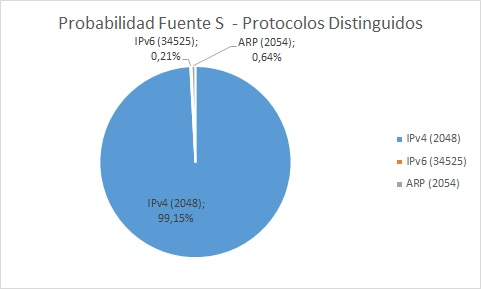
\includegraphics[width=\textwidth]{./img/probaS_casa.jpg}
\caption{Protocolos Distinguidos - Fuente S - Hogar}
\end{figure}
\newpage

\begin{figure}[h!]
\centering
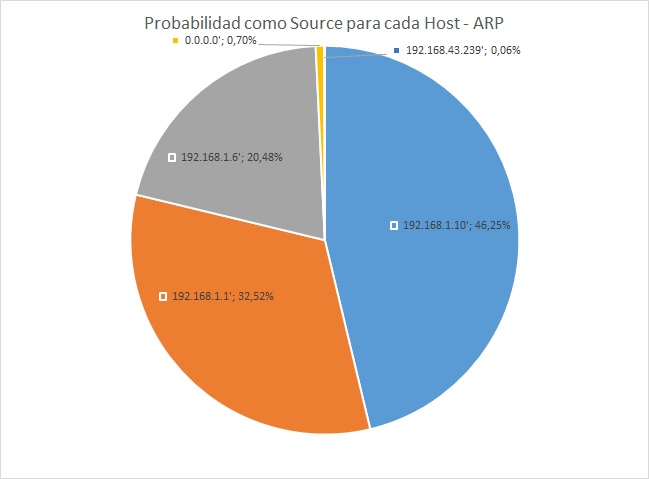
\includegraphics[width=\textwidth]{./img/proba_src_casa.jpg}
\caption{Probabilidad Source - Fuente S1(ARP) - Hogar}
\end{figure}

\begin{figure}[h!]
\centering
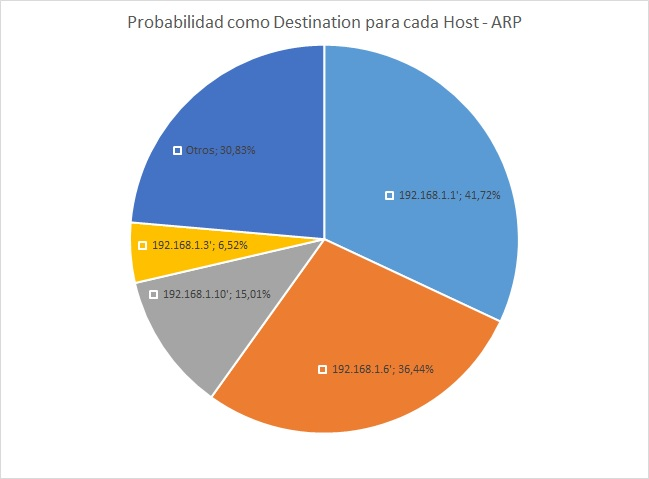
\includegraphics[width=\textwidth]{./img/proba_dst_casa.jpg}
\caption{Probabilidad Destination - Fuente S1(ARP) - Hogar}
\end{figure}
\newpage

\begin{figure}[h!]
\centering
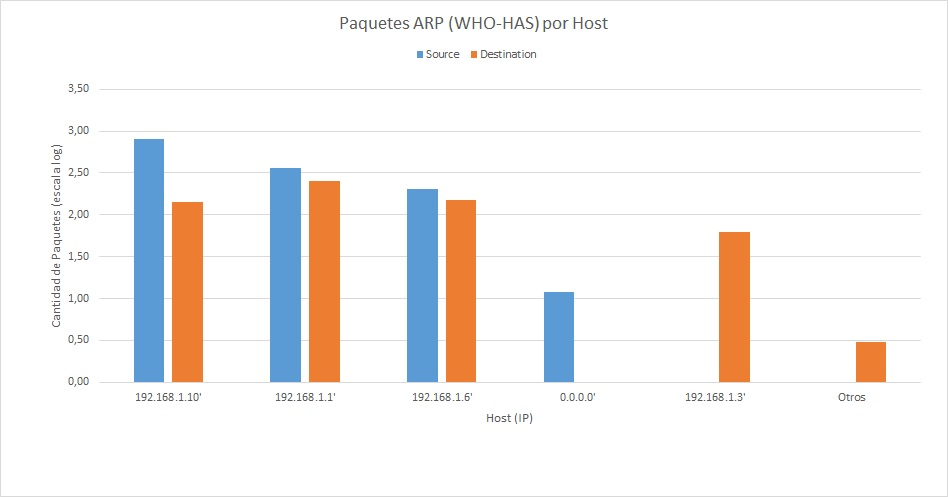
\includegraphics[width=\textwidth]{./img/arp_whoHas_casa.jpg}
\caption{Source/Destination paquetes ARP - Operación: Who-Has - Hogar}
\end{figure}

\begin{figure}[h!]
\centering
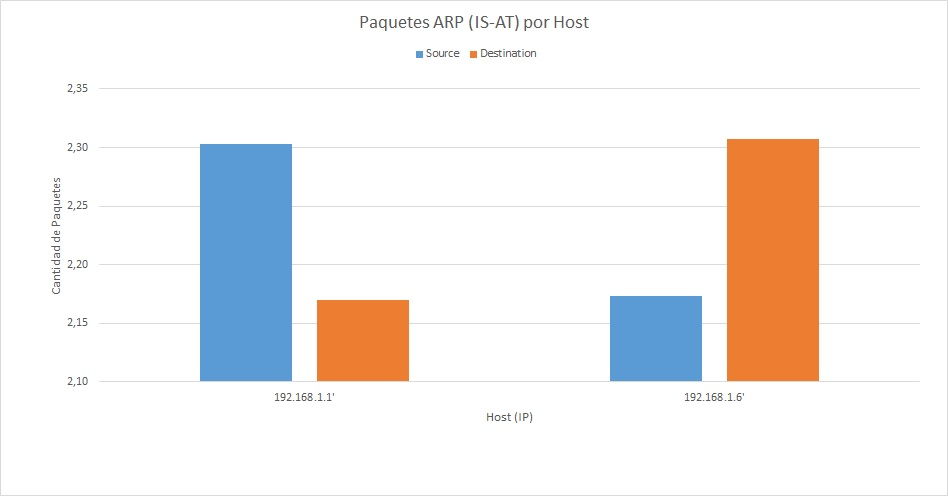
\includegraphics[width=\textwidth]{./img/arp_isAt_casa.jpg}
\caption{Source/Destination paquetes ARP - Operación: Is-At - Hogar}
\end{figure}


\begin{figure}[h!]
\centering
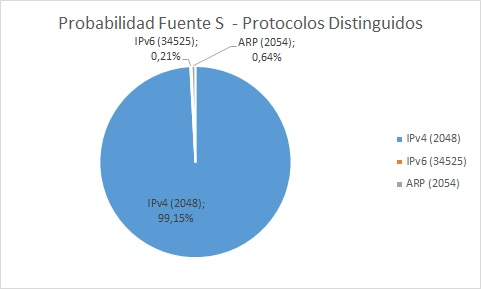
\includegraphics[scale=0.9]{./img/probaS_casa.jpg}
\caption{Protocolos Distinguidos - Fuente S - Hogar}
\end{figure}

De esta información, podemos concluir que el símbolo del protocolo $IPv4$ es mucho más probable que el símbolo del protocolo $ARP$ y que $IPv6$. 
Por lo que con lo que respecta a la fuente de información $S$, el símbolo $IPv4$ contiene mucha menos información comparado contra los otros dos. 
El cálculo de entropía de la fuente para estos datos es $0.0771$ lo que de manera intuitiva indica que la incertidumbre sobre el próximo símbolo 
de la fuente es muy baja dado que es muy probable que el próximo protocolo en aparecer sea $IPv4$.\\

Sobre la misma escucha, como ya adelantamos, simulamos la fuente de información $S1$. 
La entropía de la fuente $S1$ es de $1.98$. Esto nos parece más lógico, ya que en este caso hay más símbolos en el sistema y 
además cada uno tiene una probabilidad considerable de aparecer. Aunque, como ya veremos, algunos son más probables que otros.\\

Sobre la fuente $S1$, los resultados son los que se muestran en los siguientes diagramas:

\begin{figure}[h!]
\centering
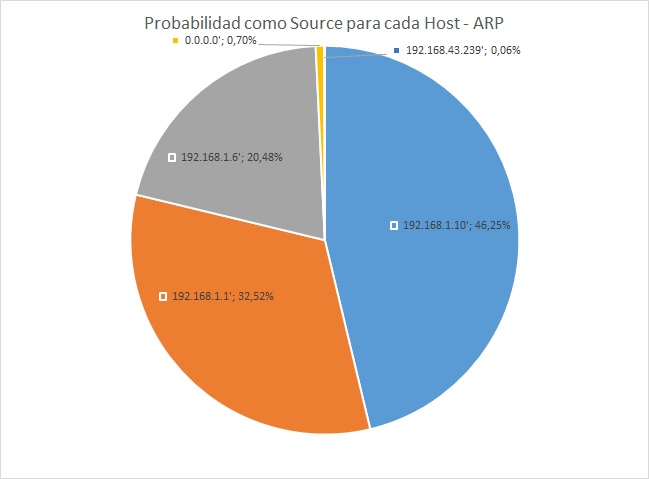
\includegraphics[scale=0.7]{./img/proba_src_casa.jpg}
\caption{Probabilidad Source - Fuente S1(ARP) - Hogar}
\end{figure}

\begin{figure}[h!]
\centering
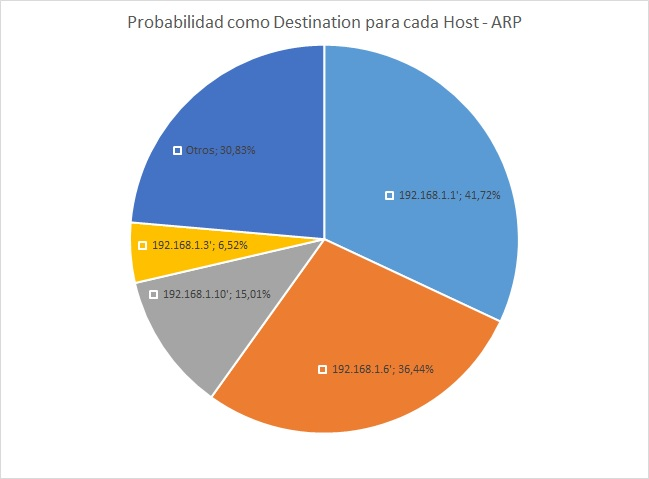
\includegraphics[scale=0.7]{./img/proba_dst_casa.jpg}
\caption{Probabilidad Destination - Fuente S1(ARP) - Hogar}
\end{figure}
\newpage

Sobre esta fuente se deben mencionar varias particularidades observadas que resultan interesantes:

\begin{itemize}
\item{La computadora con $IP$ asignada 192.168.1.10 en cierto momento realiza un escaneo sistemático de toda la red local, preguntando 
para cada ip dentro del rango 192.168.1.1-254 a quién pertenece la $MAC$. El equipo en cuestion es una computadora personal con Windows 7 instalado 
y nos resultó sorprendente observar este comportamiento para una computadora personal. 
La única explicación a la que pudimos llegar con respecto a esto es que la computadora se encuentra afectada por algún tipo de aplicación 
de bajo o alto nivel que intenta obtener información de la red local. No esperábamos este resultado este resultado para este dspositivo en particular.}

\item{Al preguntar algún host por la computadora con ip 192.168.1.36 (que se encuentra conectada por un cable ethernet al router) 
el router responde a la red wifi con su propia dirección $MAC$. En este sentido, el router estaría actuando como un bridge dentro de la red local.}

\item{El router (192.168.1.1) es el nodo que más se distingue dentro de la red. Es el que mayor interacción tiene en enviar y recibir 
paquetes $ARP$. Esto era de esperarse dado que es el host al que todos los otros preguntan dado que es el host a través del cuál 
todos los demás dispositivos acceden a Internet. El router necesita establecer y mantener actualizadas las direcciones $IP$ con las $MAC$ para
garantizar cierta fluidez en las comunicaciones.}

\end{itemize}

A continuación con toda la información obtenida, pueden observarse quiénes son los dispositivos que hacen más $Who-Has$ (azul) y 
cuáles son los dispositivos por los que más se hace $Request$ de $Who-Has$ (naranja):
\newpage

\begin{figure}[h!]
\centering
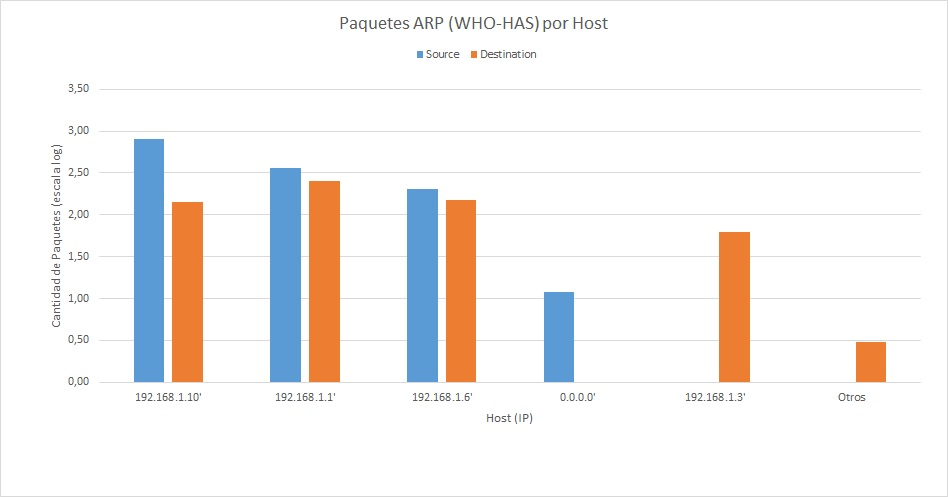
\includegraphics[scale=0.5]{./img/arp_whoHas_casa.jpg}
\caption{Source/Destination paquetes ARP - Operación: Who-Has - Hogar}
\end{figure}

De igual manera, cuáles son los que hacen más $Is-At$ (azul) y para quién está destinado el $Is-At$ (naranja):

\begin{figure}[h!]
\centering
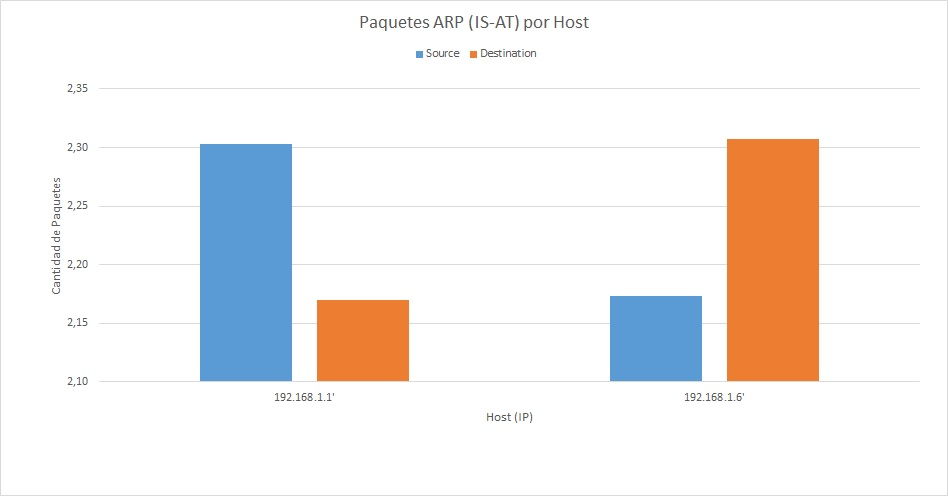
\includegraphics[scale=0.5]{./img/arp_isAt_casa.jpg}
\caption{Source/Destination paquetes ARP - Operación: Is-At - Hogar}
\end{figure}

De estos gráficos no ha llamado la atención el envío de paquetes $ARP$ de la $IP$ $0.0.0.0$. Son paquetes de operación $Who-Has$ al host
192.168.1.10 solamente. También figura con una interacción alta la $IP$ 192.168.1.6 pero se debe comunicaciones con el router que le envía
continuamente paquetes $ARP$ consultado por su $MAC$ y la computadora 192.168.1.6 responde de manera automática. Esto también nos ha llamado la 
atención dado que si bien el router recibe la respuesta ($Is-At)$ del dispositivo hemos detectado que le sigue enviando $Who-Has$ para saber su $MAC$.
También observamos que el nodo 192.168.1.36 no envía paquetes $ARP$ al router, pero sabemos que esto es porque está conectada directamente
a él a través de un cable ethernet.\\

Por último, hemos generado el grafo de la red doméstica. En dicho grafo se pueden visualizar los principales aspectos 
detallados anteriormente y nos permite entender mejor la relación entre cada dispositivo en cuánto al envío y recepción de los paquetes $ARP$.
En el siguiente grafo no se muestran todas las $IP$ que le hace $Who-Has$ el host 192.168.10.6 sino las primeras y las últimas a modo de ejemplo.
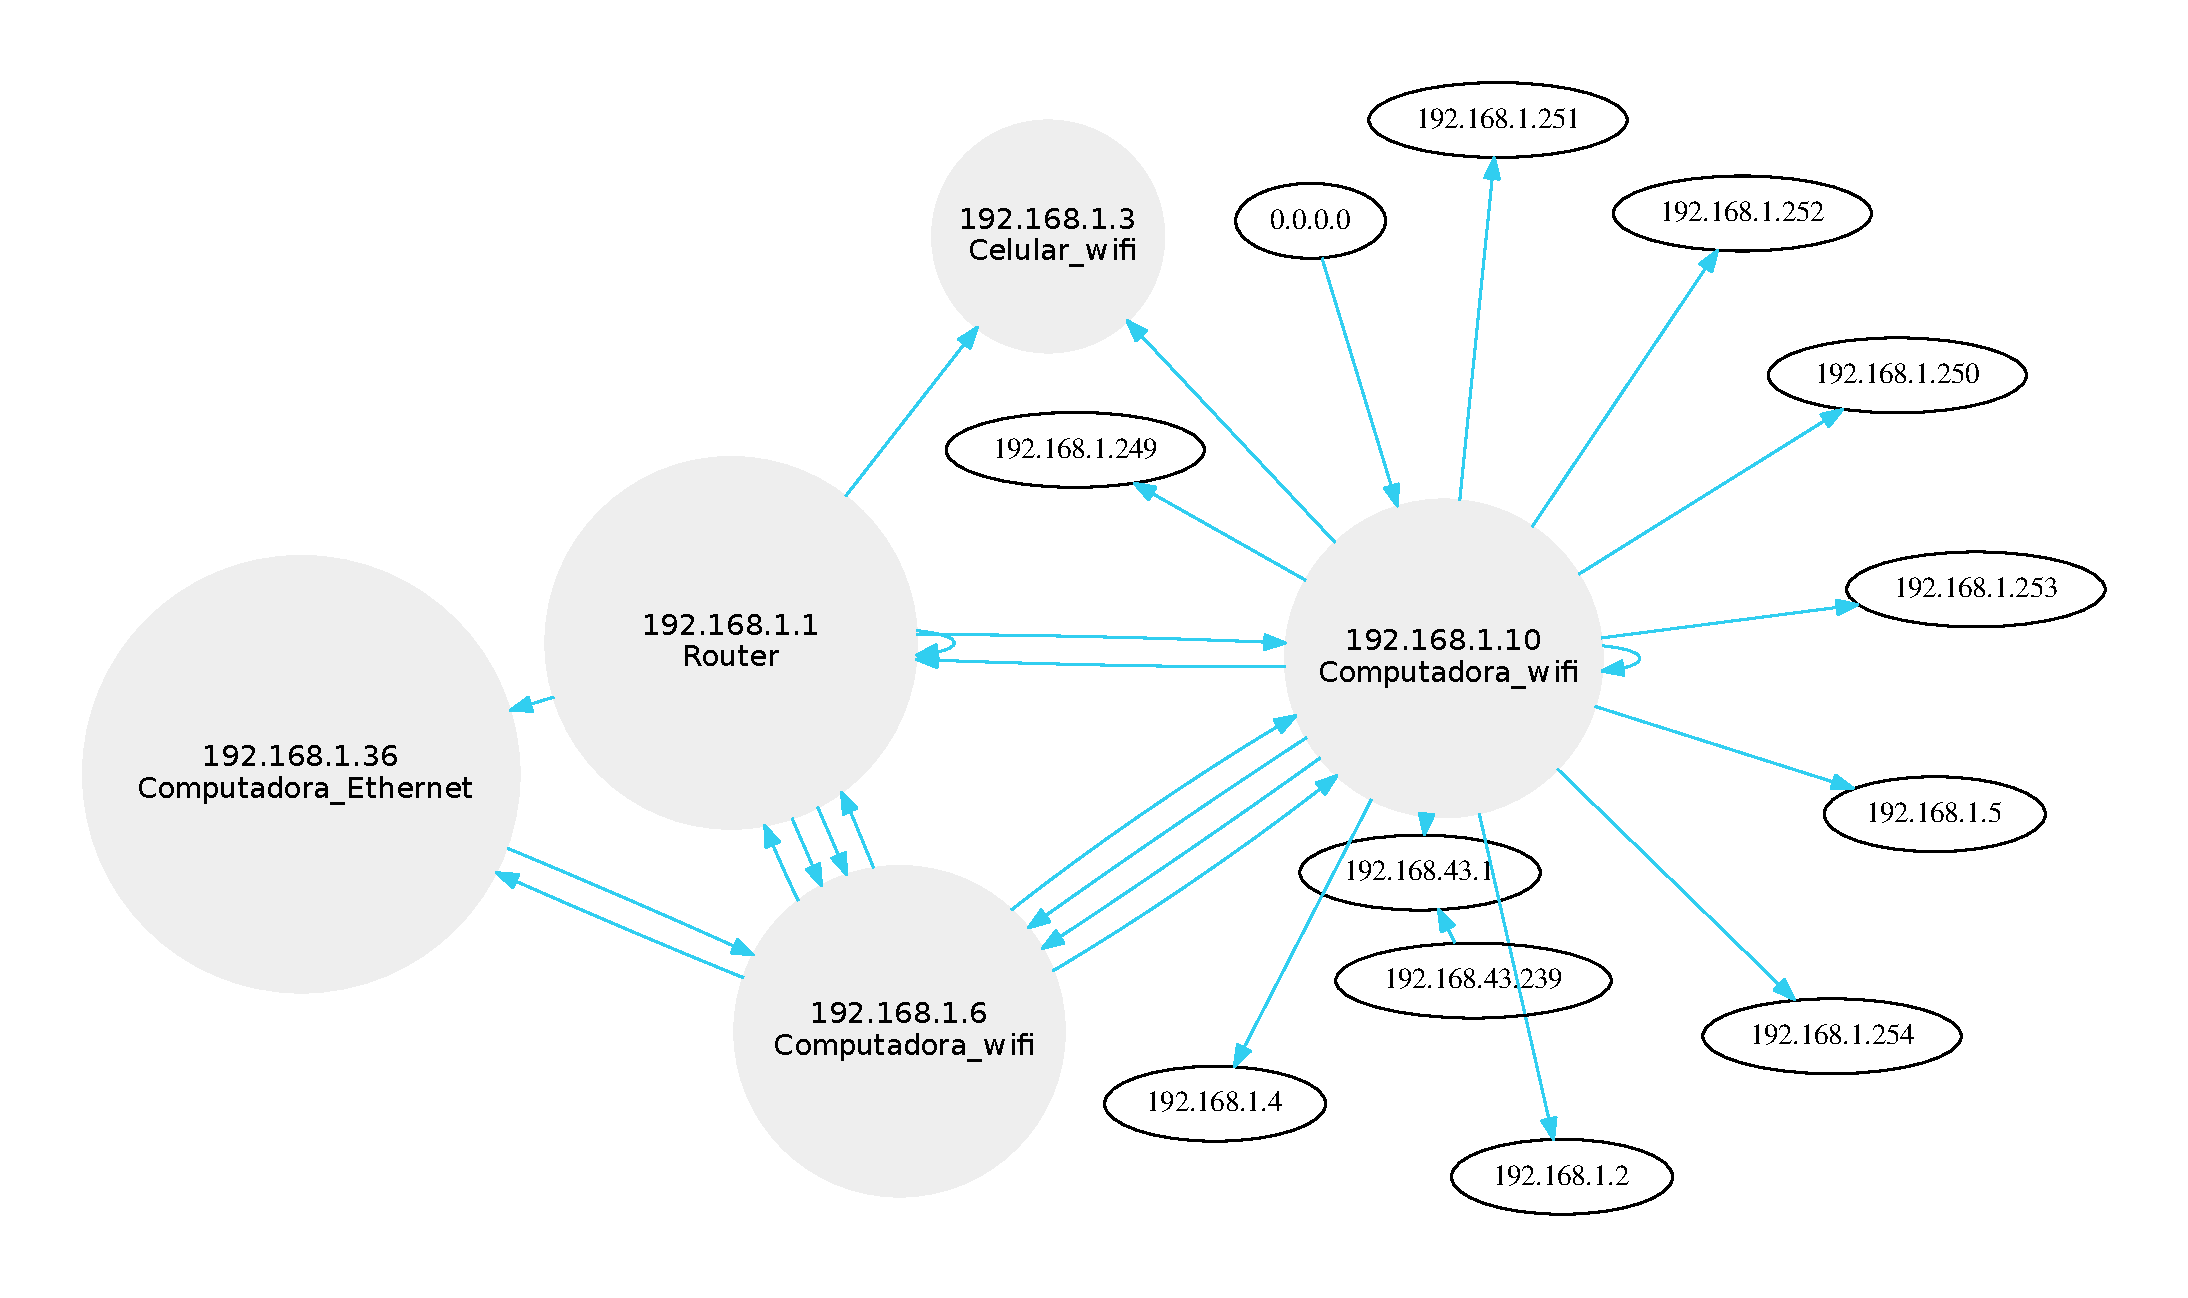
\includepdf[pages={1}]{./img/domestica_grafo.pdf}

\subsection{Redes sin información previa}
A continuación se muestra la cantidad de paquetes ARP por host en escala logarítmica. 
En el momento de realizar los gráficos, notamos que contabamos con una gran cantidad de hosts con muy baja probabilidad. 
Para mejorar la claridad y permitir apreciar los resultados a gran escala, decidimos filtrar estos casos y expresarlos como $Otros$ ya que 
no vimos valor en mostrar nodos con un 0,05 de probabilidad.\\

En las tres redes que se detallan a continuación nos hemos conectado por medio Wifi y son redes de espacios públicos sin seguridad. 
Por tal motivo cualquier dispositivo podría incorporarse a la red en cualquier momento.\\

\subsubsection{Probabilidad Protocolos - Fuente $S$}
A continuación mostramos los gráficos de Probabilidad de la fuente $S$ en las tres redes analizadas:

\begin{figure}[h!]
\centering
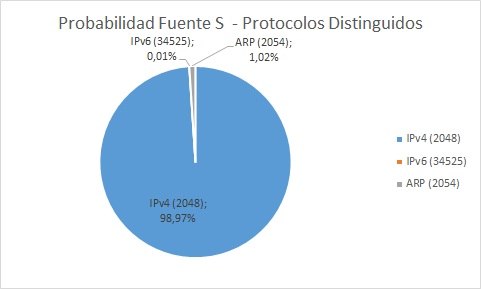
\includegraphics[scale=0.7]{./img/probaS_abasto.jpg}
\caption{Protocolos Distinguidos - Fuente S - Abasto}
\end{figure}

\begin{figure}[h!]
\centering
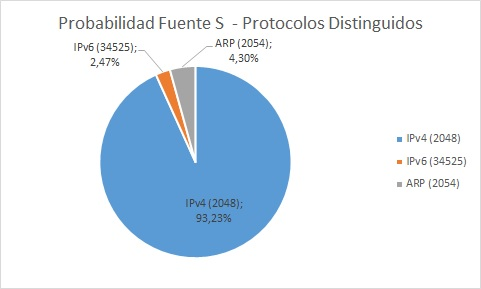
\includegraphics[scale=0.7]{./img/probaS_laboDC.jpg}
\caption{Protocolos Distinguidos - Fuente S - laboratoriosDC}
\end{figure}
\newpage

\begin{figure}[h!]
\centering
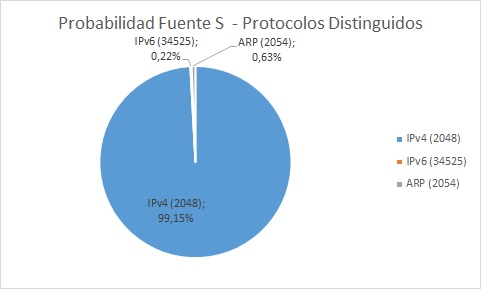
\includegraphics[scale=0.7]{./img/probaS_aulasDC.jpg}
\caption{Protocolos Distinguidos - Fuente S - aulasDC}
\end{figure}

\begin{table}[htb]
\begin{center}
\begin{tabular}{|l|l|}
\hline
Red & Entropía - Fuente $S$  \\
\hline \hline
Abasto & 0.0837 \\ \hline
laboratoriosDC & 0.4213 \\ \hline
aulasDC & 0.0774  \\ \hline
\end{tabular}
\caption{Entropía de cada Red analizada - Fuente $S$}
\label{tabla informacion}
\end{center}
\end{table}

En las redes $laboratoriosDC$ y $Abasto$ la probabilidad de paquetes con protocolo $ARP$ es mayor a la red doméstica estudiada anteriormente. 
Al ser redes abiertas y sin seguridad hay dispositivos saliendo e ingresando constantemente de las redes. Este motivo, sumado además a que 
son espacios públicos que cubren varios metros, produce que haya más paquetes $ARP$ para ir asignando la $IP$ con la $MAC$ correspondiente.
Curiosamente esto no se ha cumplido en la red $aulasDC$. Queriendo encontrar una respuesta suponemos que la mayoría de los dispositivos de la facultad
se esta conectando a la red $laboratoriosDC$ dado que en la práctica tiene un mejor señal. Al debatirlo, uno de los integrantes del grupo aclaró que
él se conectaba a la red $laboratoriosDC$ desde las aulas y que la misma tiene una mayor prioridad en su celular que $aulasDC$ para establecer 
conexión. Nos hemos basado en este caso para explicar este hecho que nos ha llamado la atención dado que esperábamos una mayor cantidad 
(en porcentaje) de paquetes $ARP$ en dicha red. Cuánto mayor es el porcentaje de los paquetes $ARP$ mayor es la entropía de las redes dado que 
no hemos detectado otros protocolos aparte de los tres detallados. Al haber más paquetes $ARP$ tenemos una mayor incertidumbre sobre el protocolo
del próximo paquete.\\

\newpage
\subsubsection{Fuente $S1$ - Paquetes $ARP$}

\textbf{Abasto Shopping}
\begin{figure}[h!]
\centering
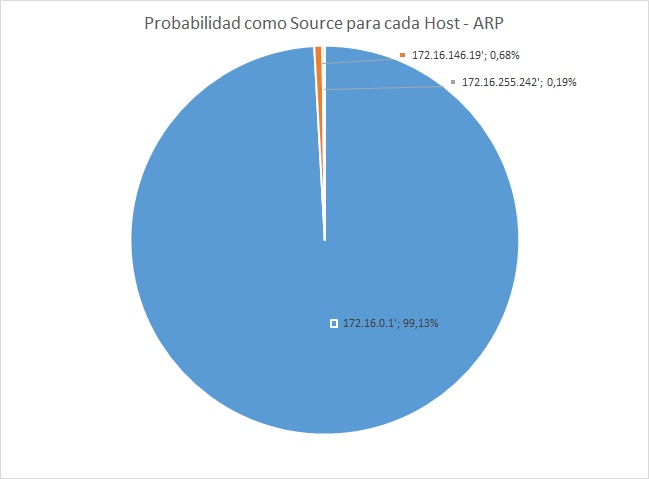
\includegraphics[scale=0.6]{./img/proba_src_abasto.jpg}
\caption{Probabilidad Source - Fuente S1(ARP) - Abasto}
\end{figure}

\begin{figure}[h!]
\centering
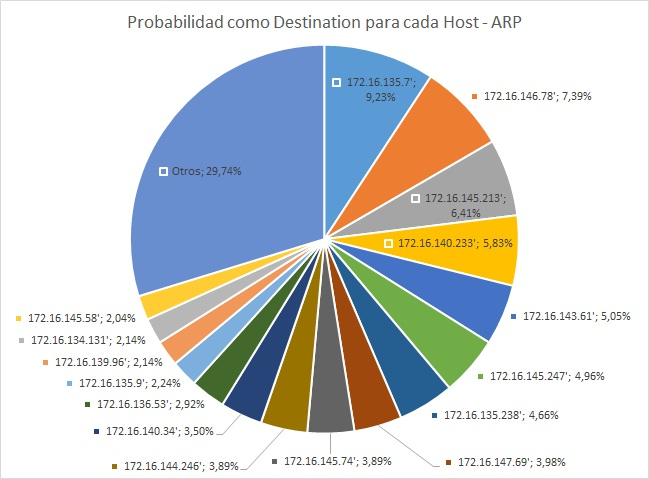
\includegraphics[scale=0.6]{./img/proba_dst_abasto.jpg}
\caption{Probabilidad Destination - Fuente S1(ARP) - Abasto}
\end{figure}
\newpage

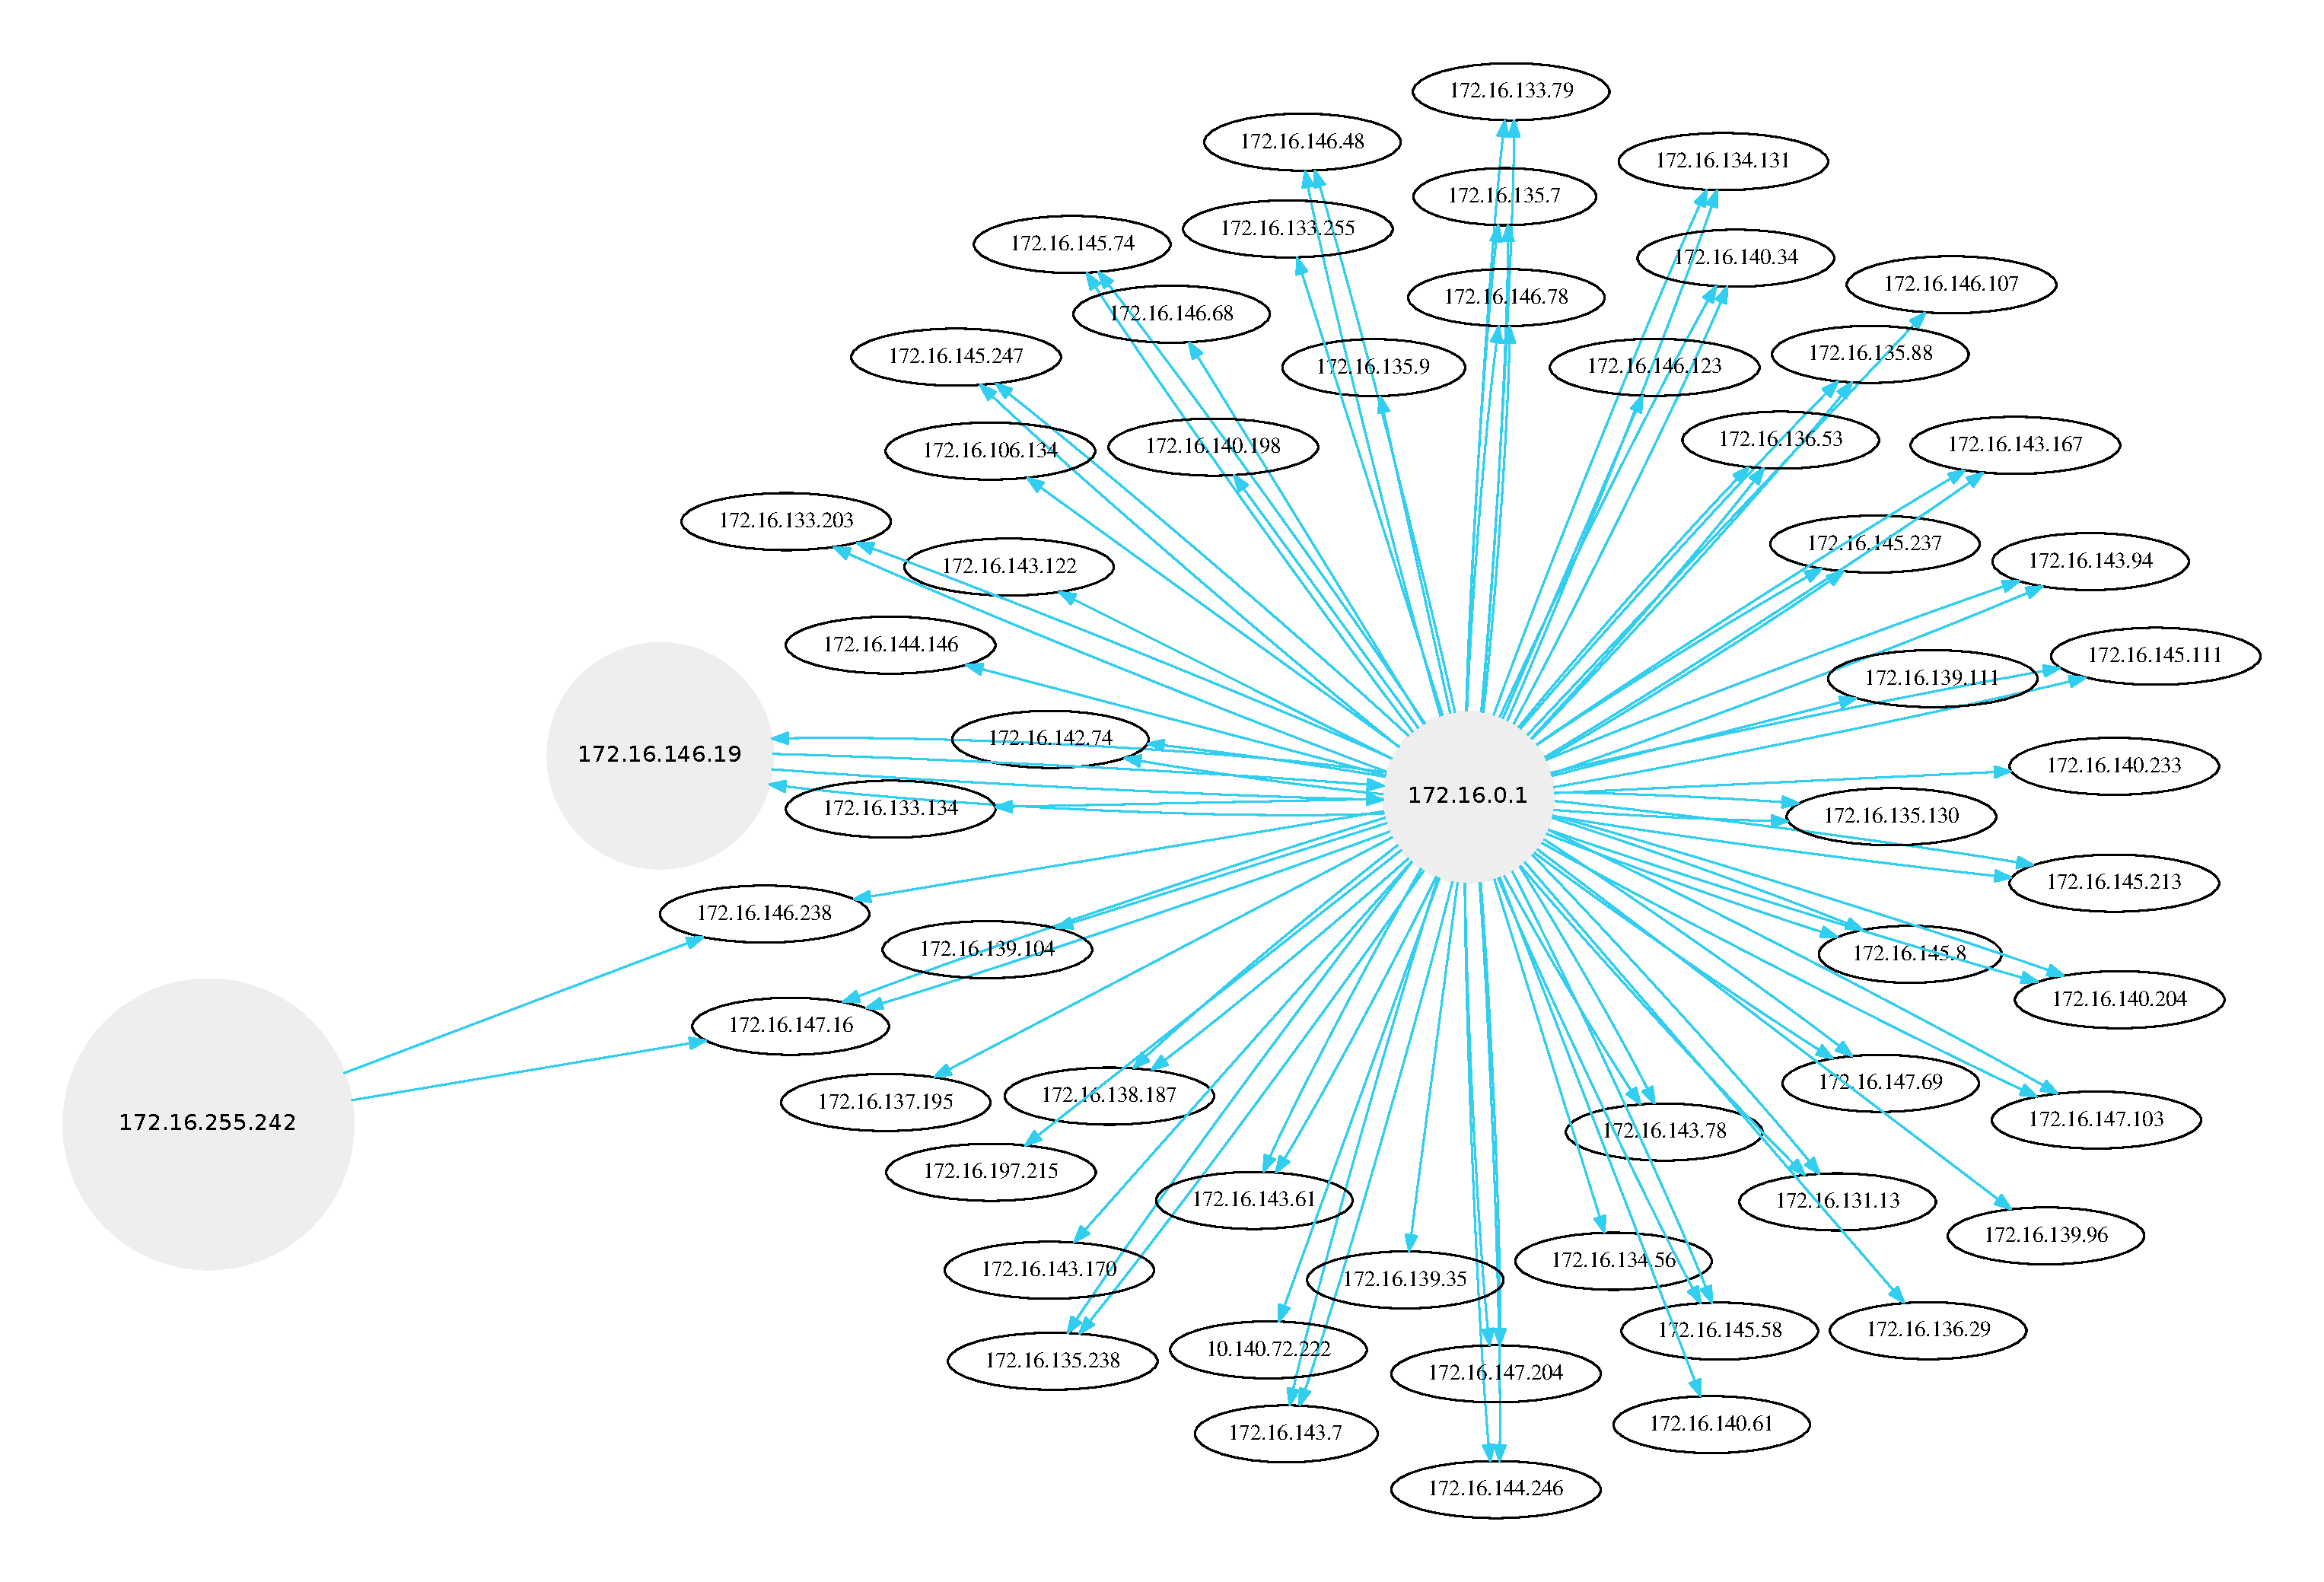
\includepdf[pages={1}]{./img/abasto_grafo.pdf}

\begin{figure}[h!]
\centering
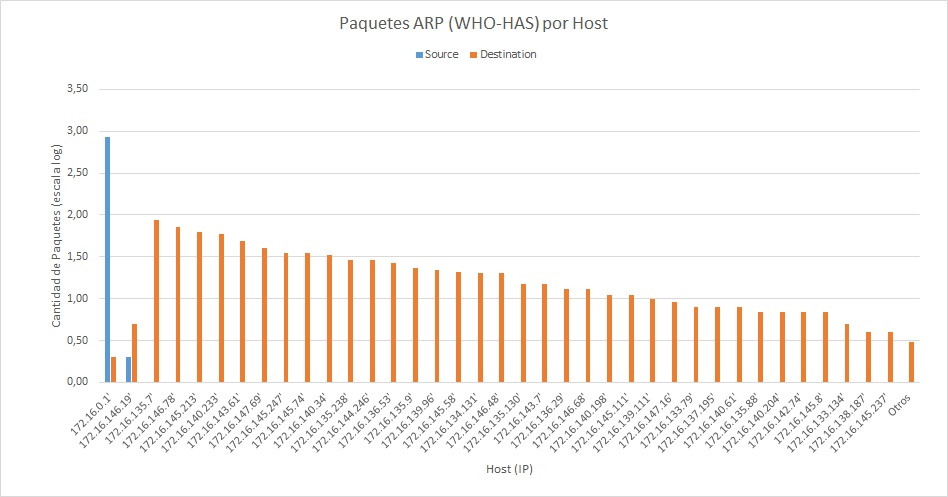
\includegraphics[scale=0.7]{./img/arp_whoHas_abasto.jpg}
\caption{Source/Destination paquetes ARP - Operación: Who-Has - Abasto}
\end{figure}

\begin{figure}[h!]
\centering
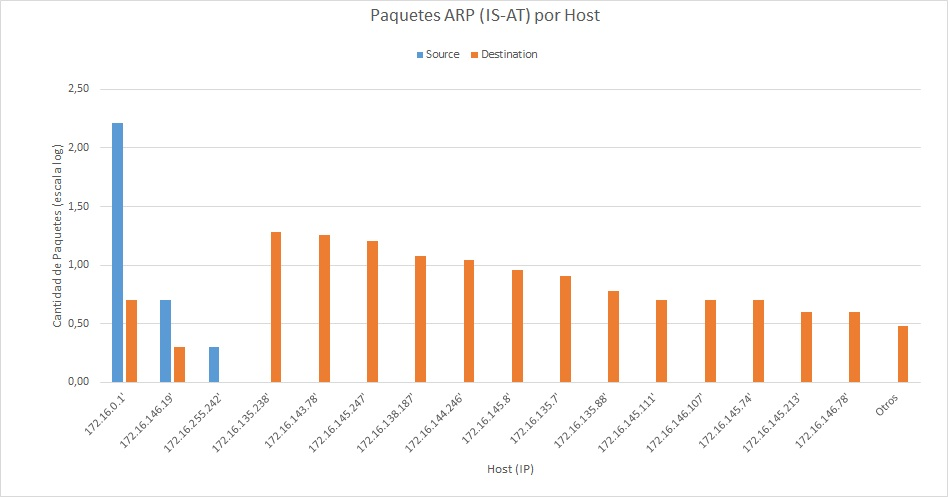
\includegraphics[scale=0.7]{./img/arp_isAt_abasto.jpg}
\caption{Source/Destination paquetes ARP - Operación: Is-At - Abasto}
\end{figure}
\newpage

\textbf{laboratoriosDC}
\begin{figure}[h!]
\centering
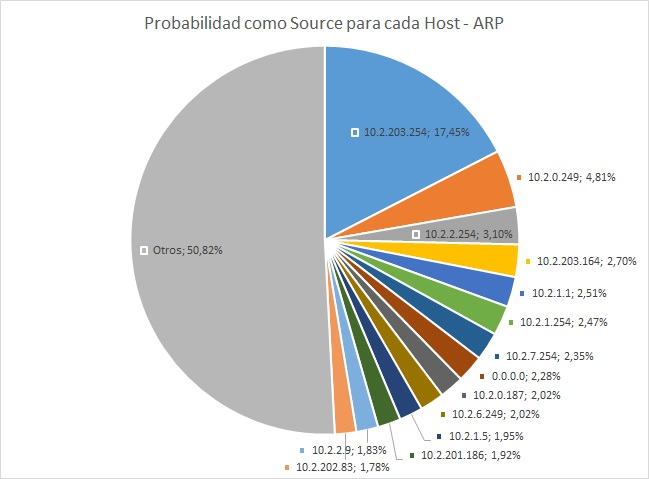
\includegraphics[scale=0.6]{./img/proba_src_laboDC.jpg}
\caption{Probabilidad Source - Fuente S1(ARP) - laboratoriosDC}
\end{figure}

\begin{figure}[h!]
\centering
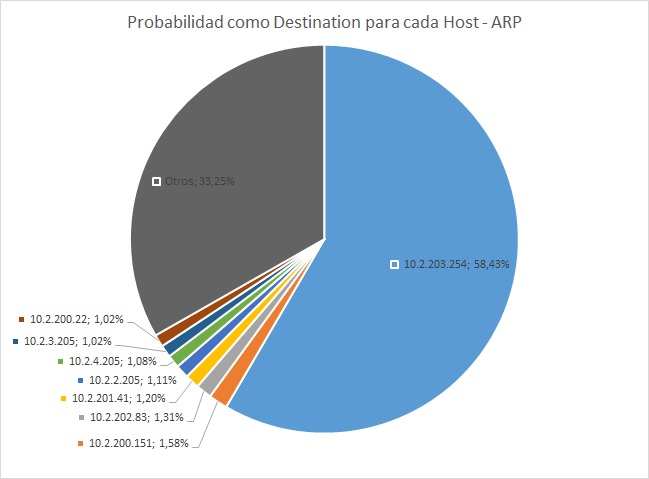
\includegraphics[scale=0.6]{./img/proba_dst_laboDC.jpg}
\caption{Probabilidad Destination - Fuente S1(ARP) - laboratoriosDC}
\end{figure}
\newpage

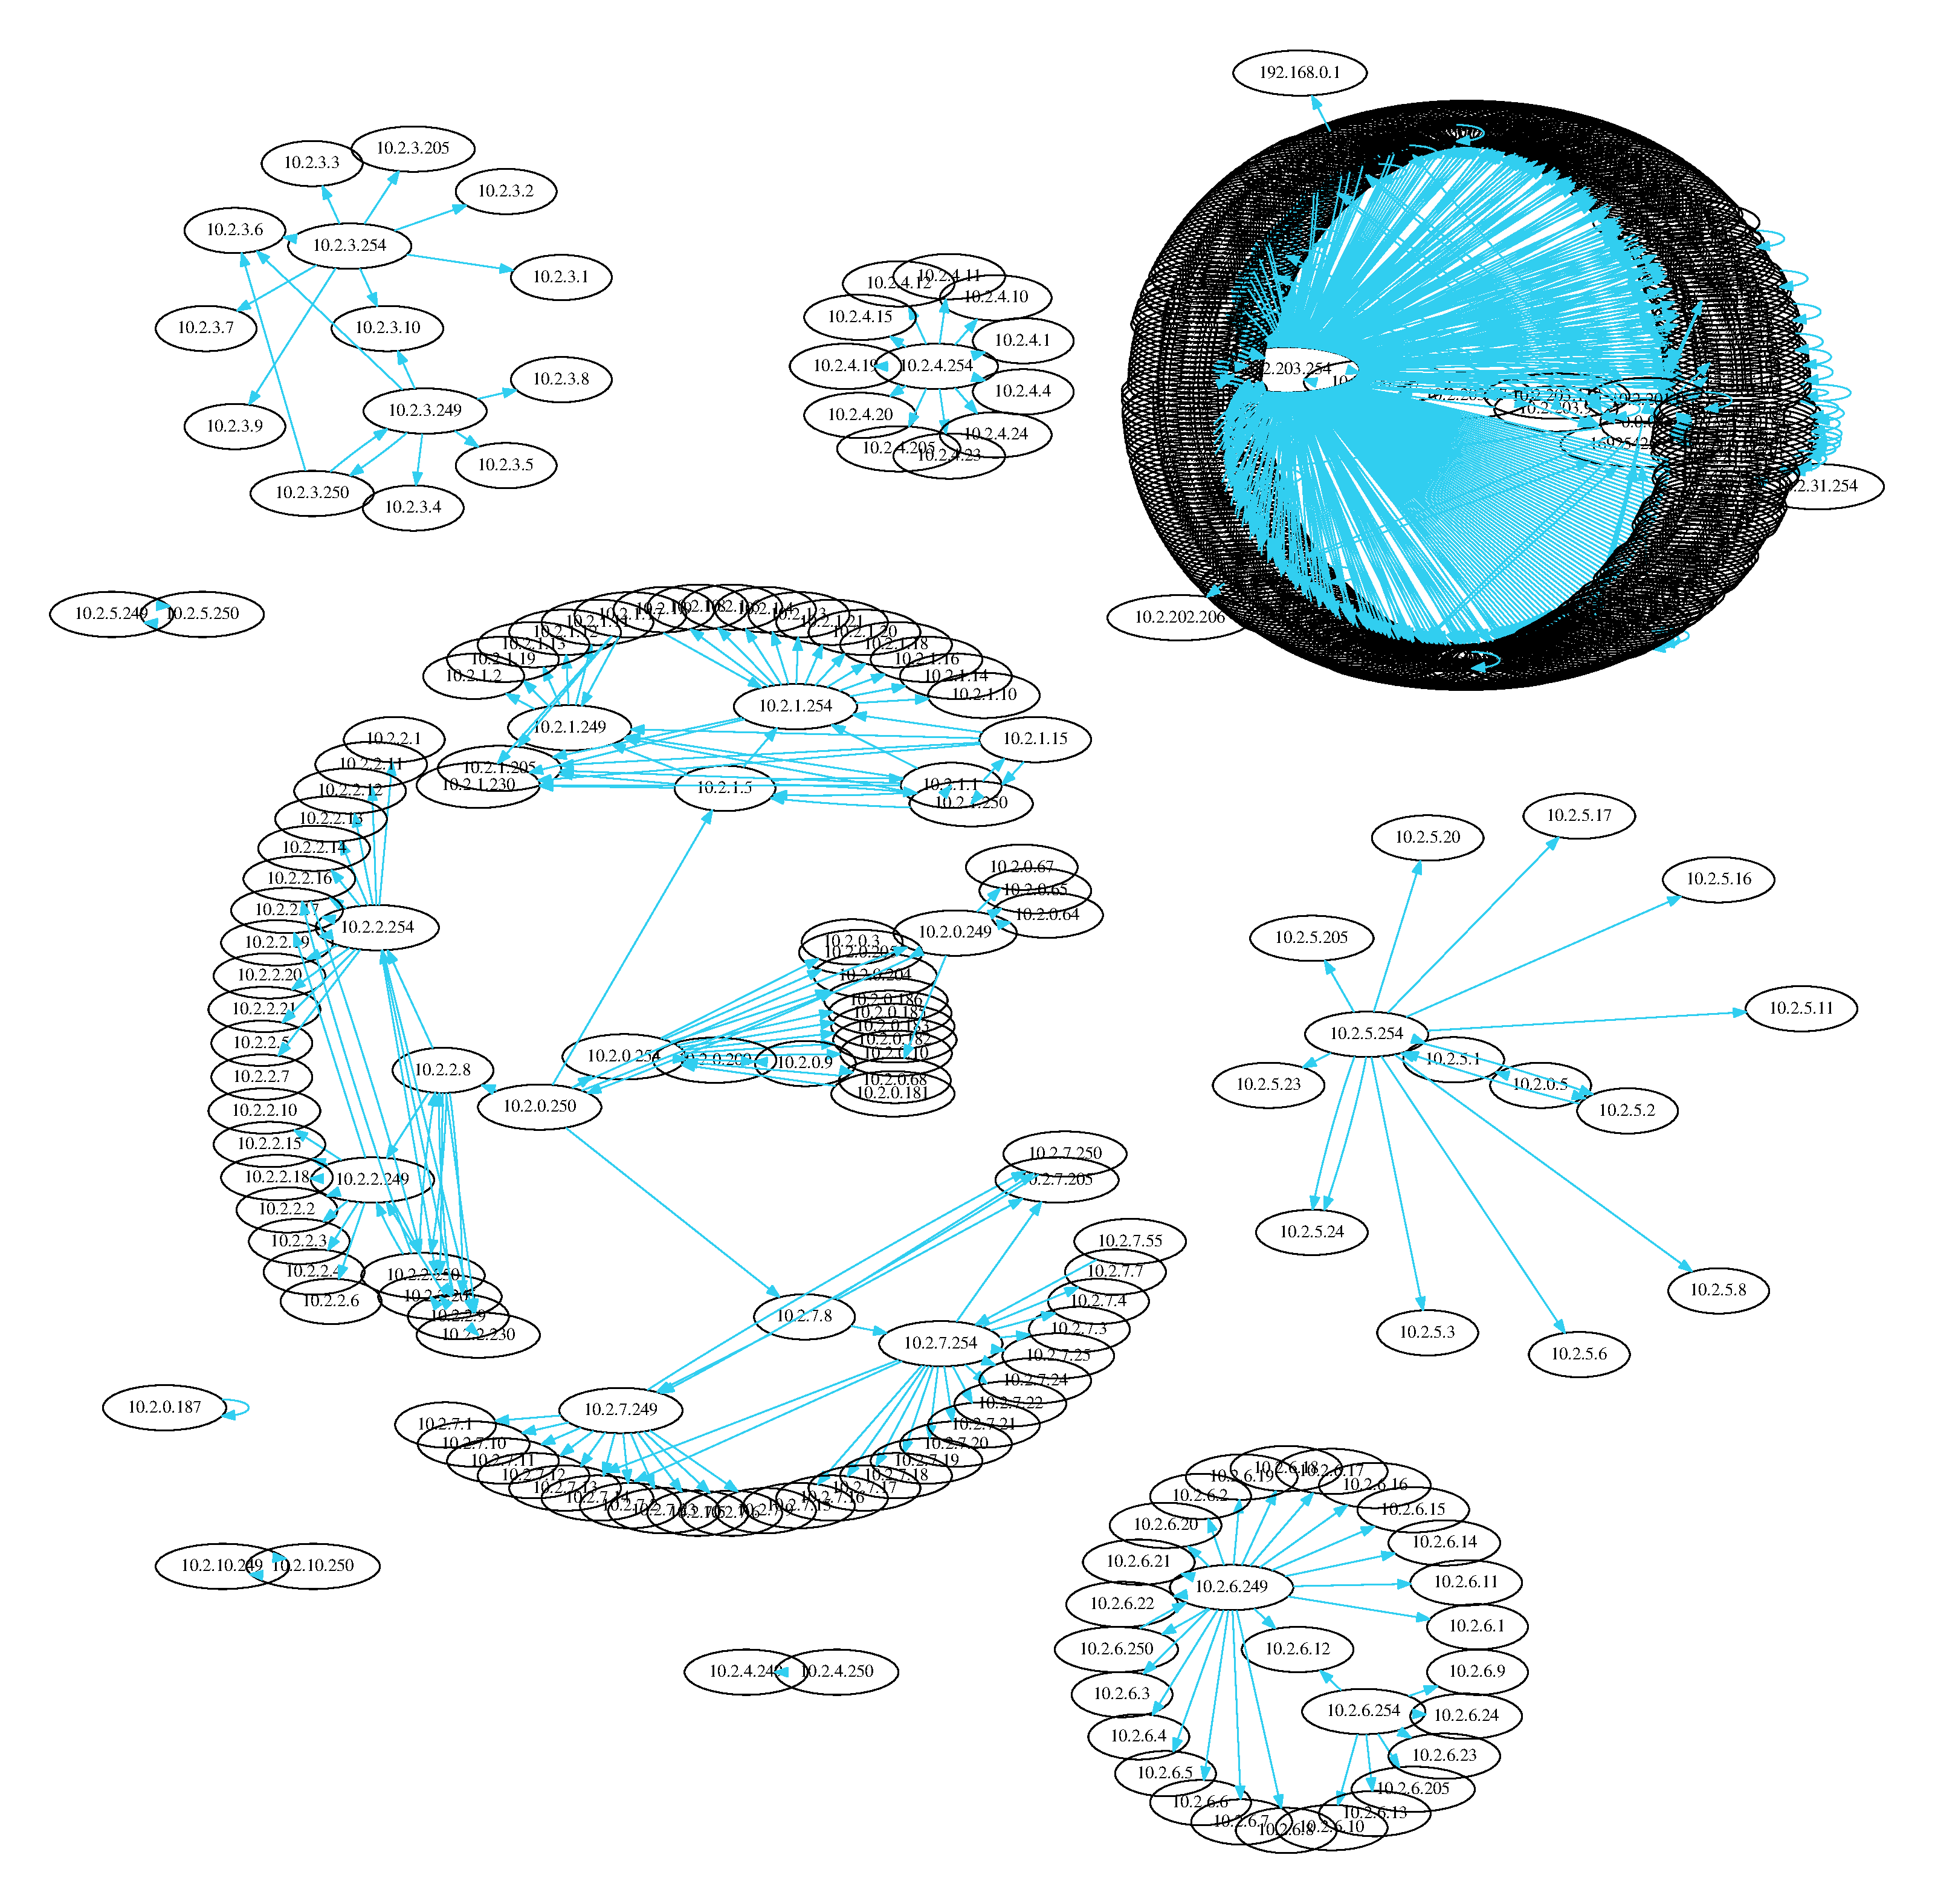
\includepdf[pages={1}]{./img/laboDC_grafo.pdf}

\begin{figure}[h!]
\centering
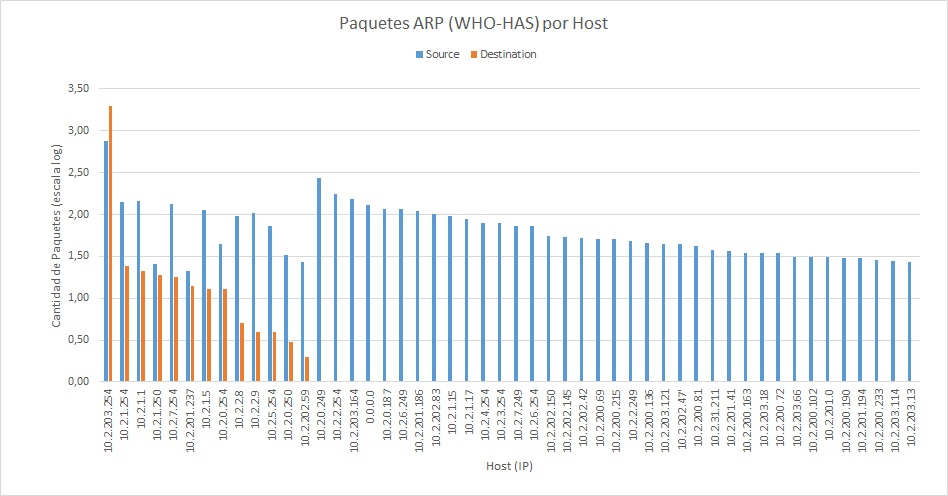
\includegraphics[scale=0.7]{./img/arp_whoHas_laboDC.jpg}
\caption{Source/Destination paquetes ARP - Operación: Who-Has - laboratoriosDC}
\end{figure}

\begin{figure}[h!]
\centering
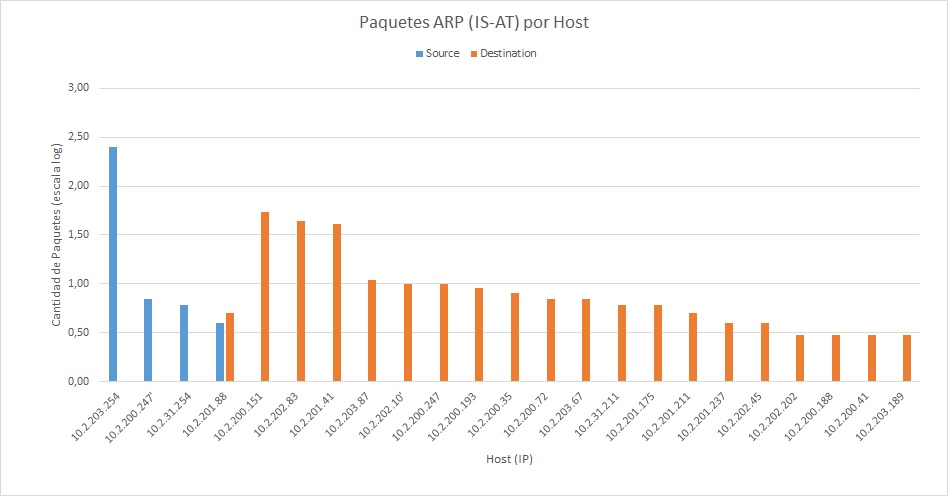
\includegraphics[scale=0.7]{./img/arp_isAt_laboDC.jpg}
\caption{Source/Destination paquetes ARP - Operación: Is-At - laboratoriosDC}
\end{figure}
\newpage

\textbf{aulasDC}
\begin{figure}[h!]
\centering
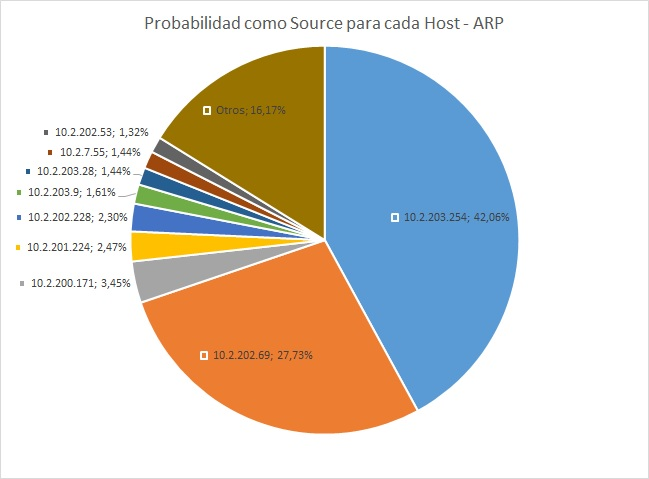
\includegraphics[scale=0.6]{./img/proba_src_aulasDC.jpg}
\caption{Probabilidad Source - Fuente S1(ARP) - aulasDC}
\end{figure}

\begin{figure}[h!]
\centering
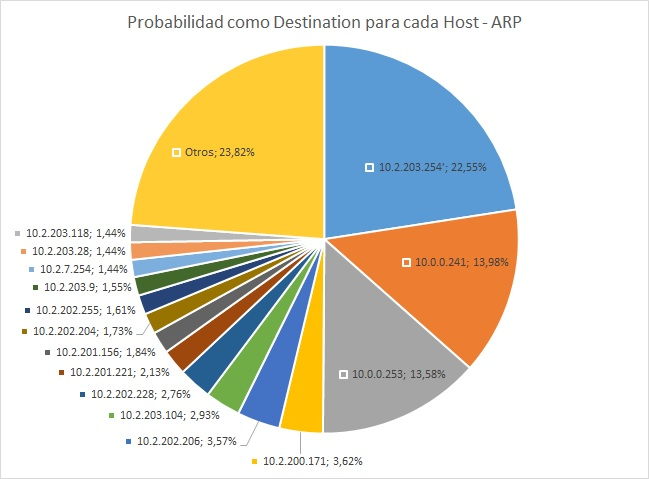
\includegraphics[scale=0.6]{./img/proba_dst_aulasDC.jpg}
\caption{Probabilidad Destination - Fuente S1(ARP) - aulasDC}
\end{figure}
\newpage

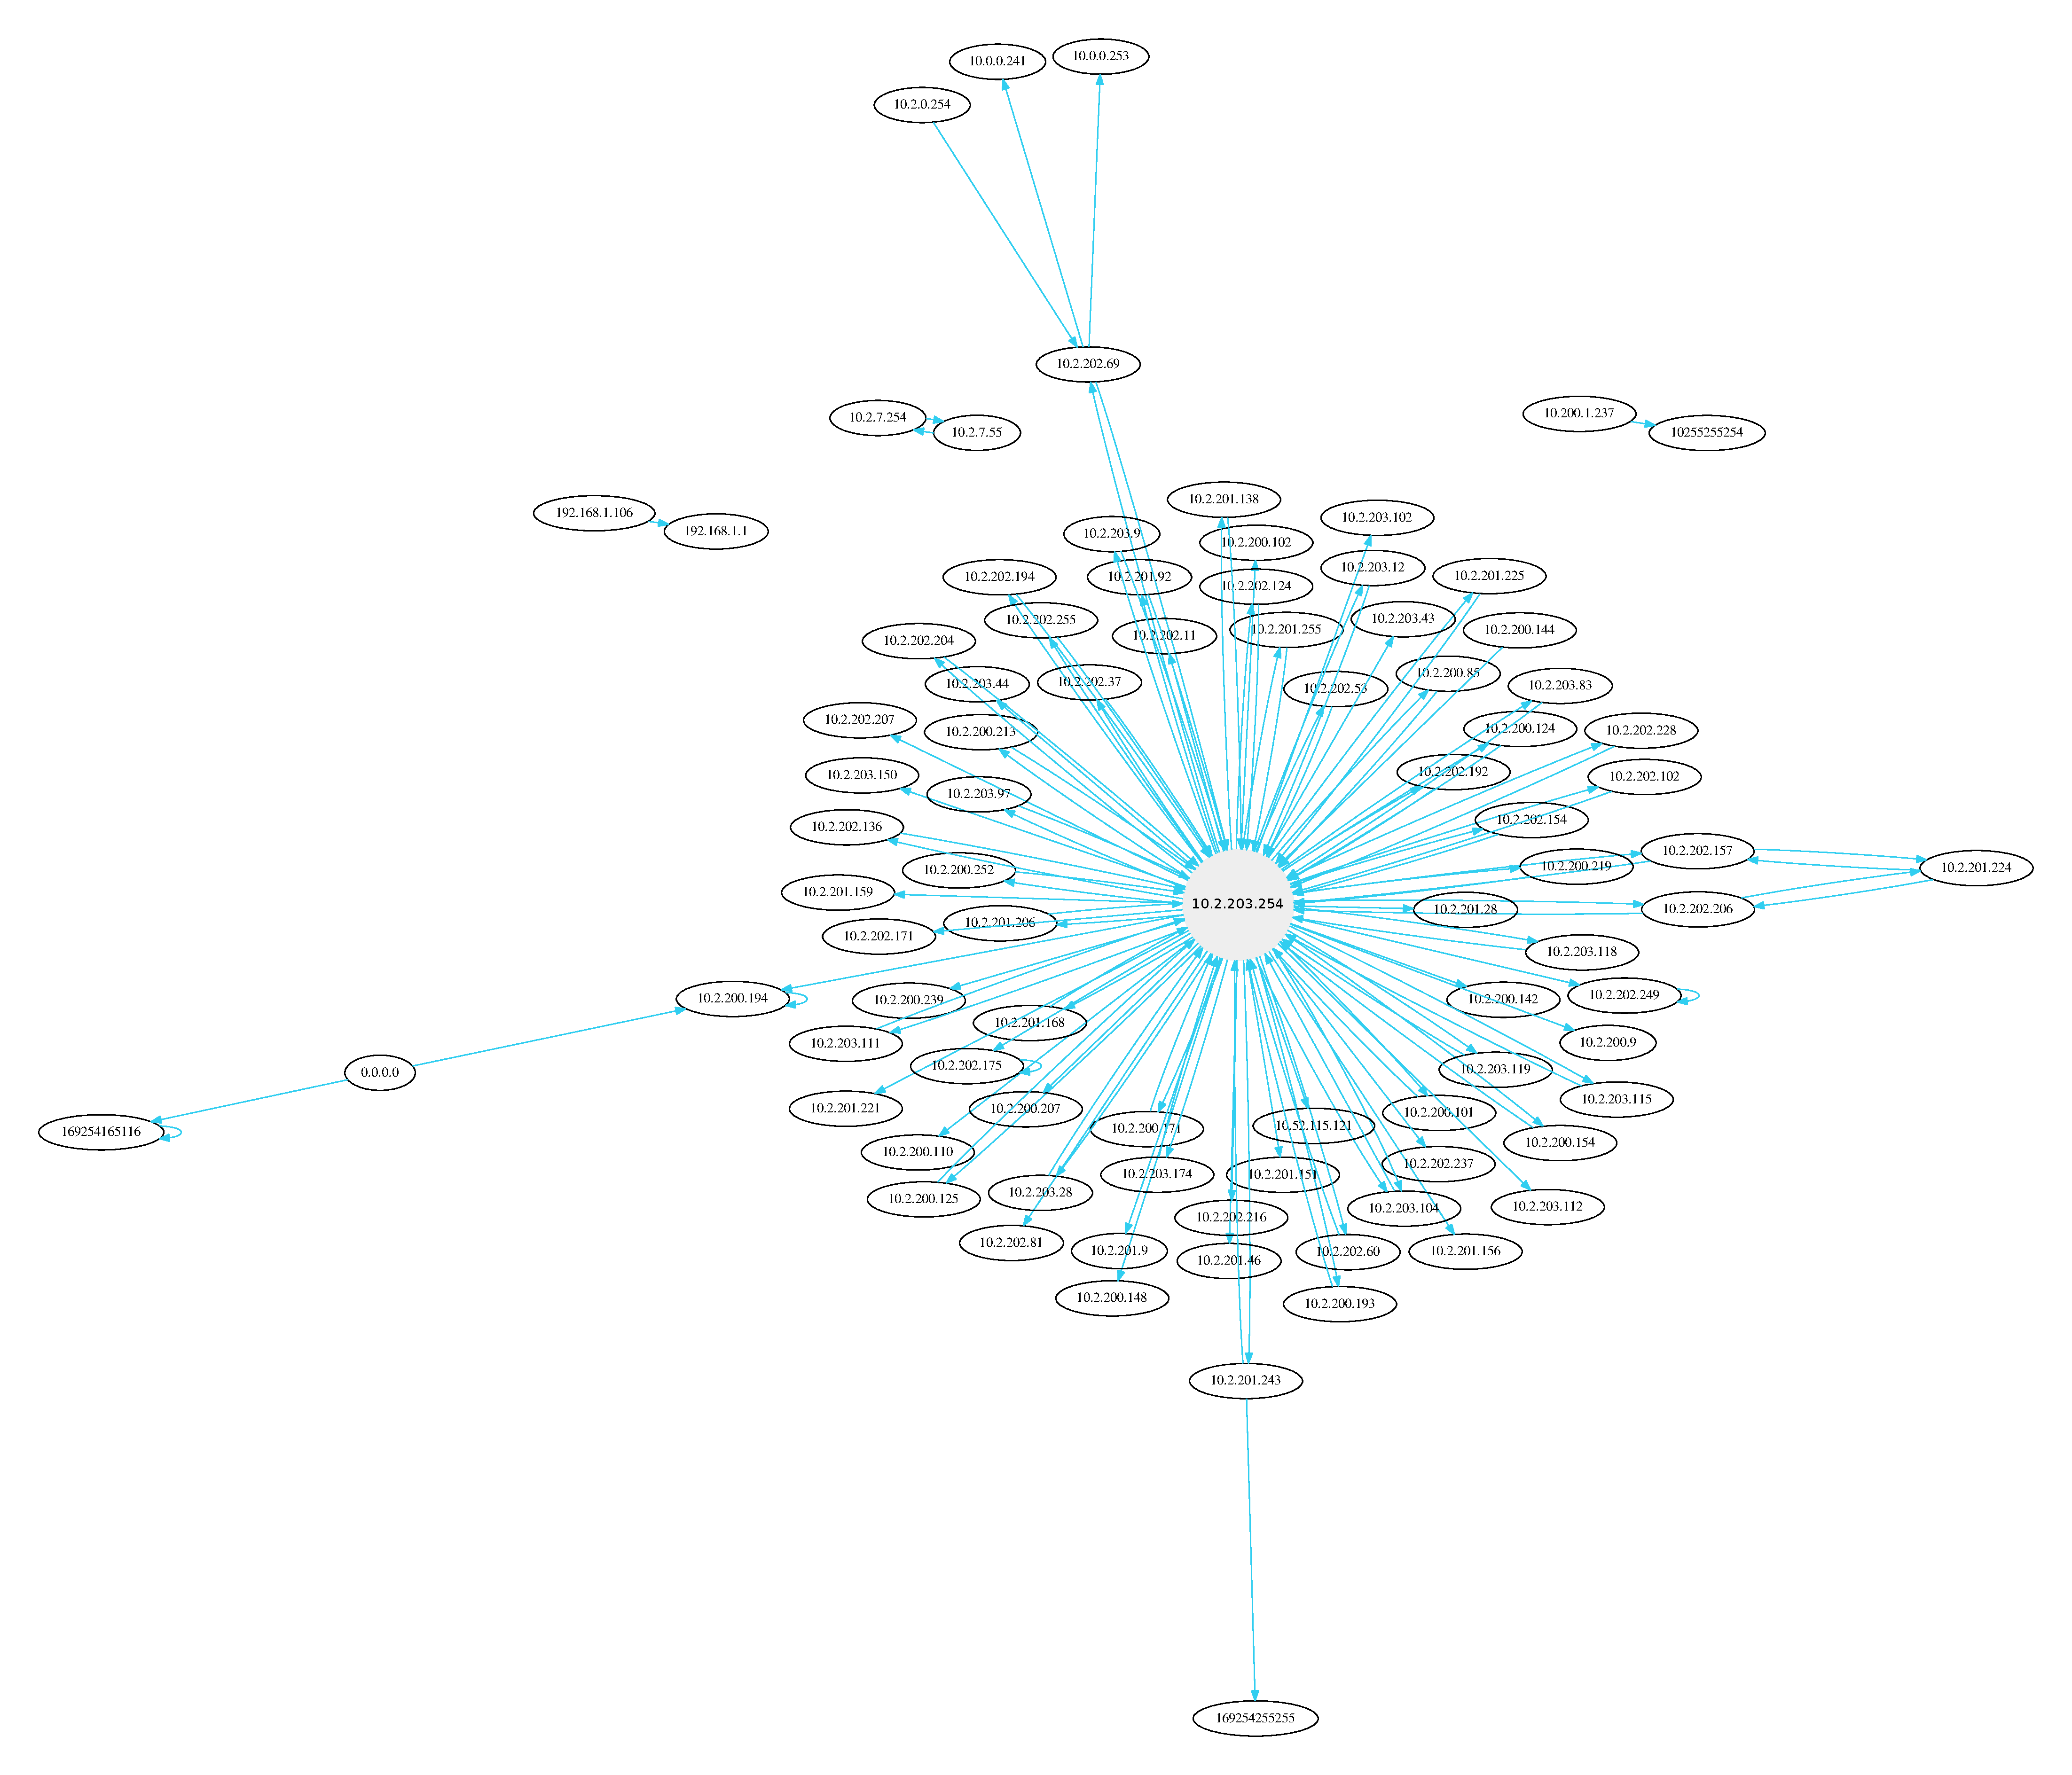
\includepdf[pages={1}]{./img/aulasDC_grafo.pdf}

\begin{figure}[h!]
\centering
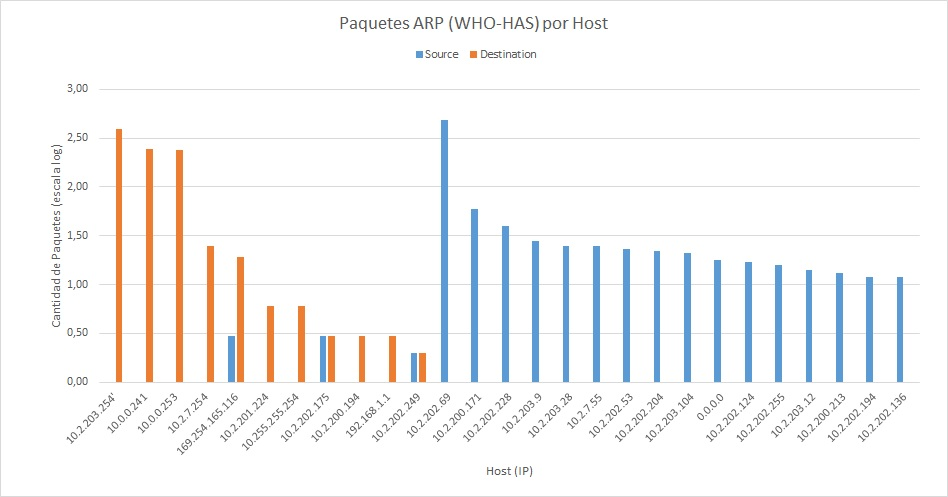
\includegraphics[scale=0.7]{./img/arp_whoHas_aulasDC.jpg}
\caption{Source/Destination paquetes ARP - Operación: Who-Has - aulasDC}
\end{figure}

\begin{figure}[h!]
\centering
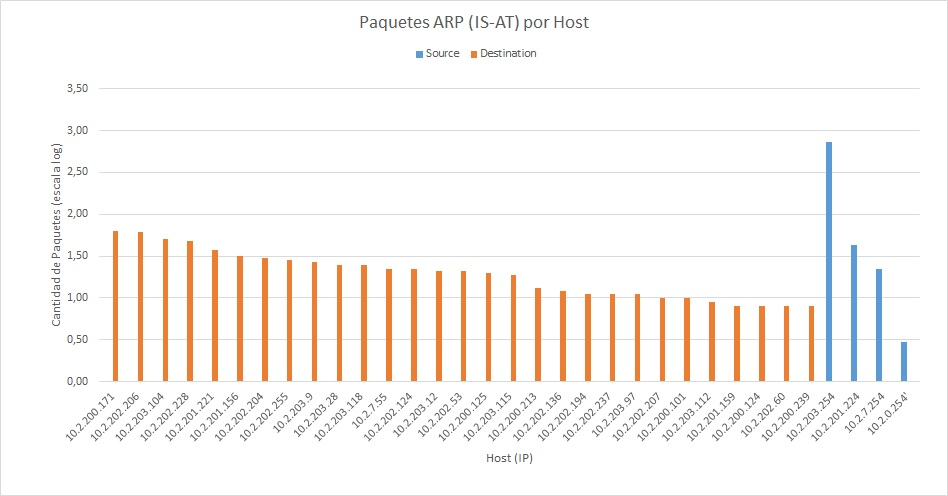
\includegraphics[scale=0.7]{./img/arp_isAt_aulasDC.jpg}
\caption{Source/Destination paquetes ARP - Operación: Is-At - aulasDC}
\end{figure}

\newpage
%Aca va frutaaaaaaaaa....
En la red $Abasto$ notamos un host que se distingue del resto: 172.16.0.1. Este host es la fuente del 99\% de los paquetes $ARP$ escuchados.
Cómo se puede ver en el grafo es el centro de la red enviando a todos los demás dispositivos $Who-Has$ para actualizar su tabla que asocia $IP$ con 
$MAC$. Analizando este comportamiento creemos que este host es el router de la red. Al enviar los $Who-Has$ a todos los dispositivos a estos no 
les hace falta consultar por la $MAC$ del router dado que al escuchar el $Who-Has$ correspondiente vinculan la $IP$ del router con su $MAC$. Otro nodo 
distinguido de la red es la $IP$ 172.16.146.19 que se comunica solamente con el que nosotros creemos que es el router. 
Seguramente sus paquetes $ARP$ se deban a una mala conexión e intenta establecer una conexión en reiteradas oportunidades. 
Otra opción es que 172.16.0.1 sea el gateway de la red y el router sea 172.16.146.19 dado que se comunica solamente con el gateway que a su vez
se comunica con el resto de los dispositivos.\\
Los demás nodos no nos han llamado la atención dado que se comunican con el router recibiendo los $Who-Has$ y al hacerlo conocen la $MAC$ del router
para luego poder comunicarse con él o simplemente no responden al no estar con una $MAC$ asociada. 
Solamente nos parece apropiado mencionar a la $IP$ 172.16.255.242 que envía $Is-At$ a dos dispositivos para establercer alguna conexión. Nos parece
raro no haber escuchado los $Who-Has$ correspondientes a esas respuestas pero podrían ser dispositivos que se encuentran muy lejos nuestro y 
no haber captado esos paquetes.\\
Lo que más no ha llamado la atención de esta red es como el router/gateway actualiza sus tablas mediante los paquetes $ARP$ enviando muchos $Who-Has$. 
Al ser una red pública y sin seguridad cualquier dispositivo se conecta aunque solo sea de paso y luego el router/gateway debe 
encargarse de establecer si esa $IP$ sigue teniendo una $MAC$ asignada.\\


El grafo de la red $aulasDC$ es muy similar a la del $Abasto$. Se puede distinguir un nodo central: 10.2.203.254. 
Este nodo recibe muchos $Who-Has$ y manda muchos $Is-At$. Esto sucede porque los demás dispostivos necesitan saber la información de este nodo.
Al recibir los $Who-Has$ de los demás nodos, no hace falta emitirlos dado que actualiza su tabla con la $MAC$ e $IP$ del emisor. Suponemos que este 
nodo es el router o gateway de la red. Aparte de este nodo nos ha llamado la atención el de $IP$ 10.2.200.69 que pregunta solo por dos disposivos
los cuales no les responden o no hemos podido escuchar sus respuestas. También hemos notado que existen muchos dispositivos solamente emitiendo o 
recibiendo paquetes $ARP$. Creemos que se debe a un mal funcionamiento de la red debido a una mala señal dentro de esta red. De la misma manera que 
en la red anterior, al ser pública puede haber muchos dispositivos conectados y por lo tanto muchas $IPs$ asignadas. Estas últimas deben actualizarse 
de manera sistemática para favorecer la conectividad y permitir unir a nuevos dispositivos.\\	


Por último en la red $laboratoriosDC$ nos hemos encontrado con un cantidad de paquetes $ARP$ que supera ampliamente a las demás redes.
Cómo nos distinguido podemos mencionar al 10.2.203.254, el cual es el 58\% del destino de los paquetes y el 17\% de la emisión de los mismos.
Al realizar el grafo de la red no hemos llevado un sorpresa. Se pueden visualizar seis subredes que se forman a partir de la comunicación de paquetes 
$ARP$. Hemos notado que cuatro subredes tiene como nodo central la siguiente $IP$ 10.2.X.254 y las mismas agrupan a los nodos que tienen $X$ en común, 
por ejemplo 10.2.5.254 agrupa los dispositivos con $IP$ 10.2.5.xxx, y el nodo 10.2.4.254 agrupa a los que tienen 10.2.4.xxx. Al meditar un poco sobre 
esta estructura y la información previa que conocemos de estas redes (dado que somos usuarios habituales de las mismas), creemos que cada subred 
pertenece a un laboratorio/oficina. Cómo no hemos podido escuchar los paquetes $ARP$ que unen todas estas subredes entre si suponemos que están 
a algún otro dispositivo por cable ethernet y con una $IP$ fija por lo cual no es actualizada. Dentro de estas redes aisladas no ha llamado la 
atención la 10.2.6.xx. En el grafo podemos ver como la 10.2.6.249 y 10.2.6.254 establecen conexiones con las demás $IPs$ y luego fluyen hacia un 
mismo nodo. Suponemos que esta red es alguna oficina y están de esta manera organizada por un tema de seguridad. También hemos hallado y vale la pena
distinguir el nodo 10.2.0.250 que une varias redes aisladas. 
Es importante notar que en el grafo estamos representado casi todos paquetes $ARP$ pero con la operación $Who-Has$. 
Este motivo, nos llevá a acentuar la idea de que cada red aislada es un laboratorio donde las computadoras están conectadas a swiches que luego 
convergen a otro dispositivo que une las redes. También deben estar conectados por cable ethernet los host 10.2.6.249 y 10.2.6.254 al host 
10.2.6.12 pues hemos escuchado los $Who-Has$ y no sus respuestas.
Solamente hemos sido testigos de los $Is-At$ que abarcan a nuestro principal nodo distinguido (10.2.203.254). 
Este último seguramente sea el router o gateway de la red de wifi dada la gran de $Ips$ con la que realiza las interacciones. 
Es importante notar que es la misma $IP$ con que nos hemos encontrado en la red $aulasDC$. Al ser redes "hermanas" 
nos inclina más a suponer que esta $IP$ es el gateway de la red siendo un nodo sumamente solicitado por los demás dispositivos y 
en constante actualización de sus tablas.\\

Por último mostramos la entropia de la fuente $S1$ de cada una de las redes.\\

\begin{table}[htb]
\begin{center}
\begin{tabular}{|l|l|}
\hline
Red & Entropía - Fuente $S1$  \\
\hline \hline
Abasto & 3.0335 \\ \hline
laboratoriosDC & 3.6584 \\ \hline
aulasDC & 3.8840  \\ \hline
\end{tabular}
\caption{Entropía de cada Red analizada - Fuente $S1$}
\label{tabla informacion}
\end{center}
\end{table}

Al haber estudiado y observado el grafo de la red $Abasto$ nos parece bastante coherente que tenga una menor entropía que las otras redes. Esto se 
debe a que existe un nodo central que, según pudimos distinguir, une toda la red. Al pasar esto la incertidumbre de la red es menor dado que 
la probabilidad que aparezca este nodo en los paquetes $ARP$ es mucho mayor a que aparezcan otros. No ha llamado la atención que esto no ocurriese 
para la red $aulasDC$ que ha sido la de mayor entropía calculada. Si bien hemos podido identificar también un noodo central, al parece hay más 
incentidumbre en cuánto a los nodos que interactúan en la red. Una suposición es que quizás la red cuente con poca señal wifi provocando que 
los dispositivos se conecten varias veces hasta establecer una conexión y cambien su $IP$ más frecuentemente. Con lo cuál las probabilidades son un 
poco más equiprobables en dicha red haciendo que la entropía sea mayor.
En la red $laboratoriosDC$ al identificar varias subredes la entropía es alta dado que existen varios nodos centrales que unen estas redes.

Por último durante las capturas, hemos identificado ciertos dispositivos con $IP$ 0.0.0.0 creemos que esto se debe a que cuando un cliente se conecta a una red que posee un servidor DHCP y quiere recibir una IP de éste, manda una petición con su ID en forma de broadcast para que lo detecte el servidor. Una vez detectado por el servidor, éste manda una o varias ofertas de IP a ese ID.
El cliente eventualmente podría recibir la oferta, tomar uno de esos IP y extraer la dirección del router.
Como el servidor realiza la misma operación con todos los demás clientes que pidan una IP, el cliente debe comprobar que la IP que eligió no la tiene otro cliente. Para esto, envía un paquete $who-has$ con su MAC adress y la IP 0.0.0.0 como fuente para evitar confundir las ARP caches en otros hosts. Si el $who-has$ es respondido, el cliente rechaza el IP elegido.

